\chapter{Predicting optimal Spark settings in standalone mode}

\emph{Abtsract} What are the optimal settings for a long running, standalone mode Spark based, stateless process? The paper investigates the effects of four different parameters and compares the application's behaviour in two different servers. The most important lessons learned in this experiment is that allocating more resource does not necessary imply better performance, moreover what we really need in an environment with limited and shared resources is a 'good enough' state which politely let other processes run. To find the optimal settings it is suggested to pick up a smaller sample, which is similar to the full dataset in important features, and measure performance with different settings. The settings worth to check are number of cores, memory allocation, compression of the source files, and reading data from different file systems (if they are available). As a source of ground truth Spark log, Spark event log, or measuring points inside the application can be used.

%\keywords{Apache Spark \and performance metrics \and metadata quality \and Europeana.}
%\end{abstract}
%
%
%
\section{Introduction}
Measuring the quality of cultural heritage metadata is a task which has two important features. First, in Digital Humanities (DH) context the size of source data (library, archives or museum (LAM) catalogues, or aggregated catalogues/datasets such as Europeana\footnote{\url{https://europeana.eu}}, Wikidata\footnote{\url{https://wikidata.org}} or Archives Portal Europe\footnote{\url{http://www.archivesportaleurope.net/}}) could be regarded as big data. Big Data is a relative concept, usually it means that the data is larger than what you could process with traditional methods within the infrastructure available in the organization. DH or even cultural heritage traditionally is not equipped with high performance computing tools, so here the volume of Big Data are smaller than for example in astrophysics, or medicine. On the other hand the variety of the data is large. Second, even after a decade of research (\cite{zotero-bibliography}), the LAM community has not yet reach a clear consensus on the exact meaning of metadata quality. We have different quality dimensions and metrics, but current researches are still experimental and in some extent based on trial and error workflow, in which metrics are selected from the literature or new metrics are invented, their measurements are implemented and tried on the (meta)data, finally metadata experts evaluate the result, and suggest changes on the measurement. The consequence of this research cycle is that it necessitates the execution of multiple long running measurements of the same big data set. Among other tools Apache Spark\footnote{\url{http://spark.apache.org/}} helps to decrease the duration of this process by letting the existing process run parallel fashion. Spark could be run in a cluster, but in a DH/LAM context clusters are rarely available, so a more typical use is to run Spark in `standalone mode' which make use the multicore architecture of a single machine and simplifies writing multithreaded software code. Commercial or scientific conference presentations about Spark performance usually concentrate on clustered environment, and one can hardly find suggestions on the standalone mode. This paper aims to suggest some easy preliminary measurement of a Spark run to find the optimal settings.

\section{Measuring completeness of Europeana records}
Europeana is a digital platform of the European cultural heritage, which aggregates catalog records from European libraries, archives, museums, and other cultural organizations (called data providers). In this research a snapshot of records were used which were created in 2018 August and contains approx. 62 million records. Each record are in Europeana Data Model (EDM)\footnote{\url{https://pro.europeana.eu/resources/standardization-tools/edm-documentation}} metadata schema, which has the several parts or `entities': a descriptive metadata part (`proxy'), and optional contextual entities which describe the agents, concepts, places and time spans mentioned in the proxy. Moreover Europeana not just aggregates these records, it enhances them as well: with the help of semantic web technologies and linked open data it tries to detect entities in the data provider's proxy, and to save them as additional contextual entities.

The data are stored in a MongoDB database. Since reading from MongoDB is time consuming process, and Spark's Mongo connector does not support a specific reference type which is heavily used in the database, we chose to export the data to text files in which every line is an individual, denormalized record (here denormalization means that the record packages together the proxies, and all linked contextual entities instead of merely keeping the references to them). The process is built on Spark's Mongo connector enhancing with some extra API calls\footnote{\url{https://github.com/pkiraly/europeana-qa-spark}}. The best part of Spark's Mongo connector, that like in the processing of text-based input files Spark makes partitions of Mongo, and able to run exporting them parallely. At the end of the process 1740 files each with 35.6 thousand records were created. The size of the files varies, their average size is 0.47 GB (the bulk is between 0.23 and 0.9 GB).

After this preparation phase comes a record level measuring part, which is based on Spark's Java API. In the project there are multiple measurements, for this experiment the \emph{completeness measurement} were selected. It takes a JSON string and checks every field in the schema whether they are available in the record and returns an integer (zero or more) denoting the number of available field instances. The result is serialized as a CSV formatted string which contains record identifiers, some selected metadata (the identifiers of sources of the records), and the fields cardinalities. Spark takes care of reading the input and writing the output, and distribution of the processing over the available CPUs. The part of the process which interacts with Spark is provided in Listing \ref{code:spark_api_usage}. The next steps are statistical analyses of the resulted CSV, which produce a set of CSV files with statistical description of the whole collection and its 20K subcollections (records belonging to the same dataset, data provider or provider, or records come from the same countries, or written in the same language -- and the combination of these), an their visualization on a web based user interface.

From Spark's perspective it is the most minimalistic use of Spark: above the mandatory input and output calls only one extra method is used: map(). It is important to know, that Spark API is similar to SQL queries that it is high level API, and the engine behind optimizes it and creates a low level implementation. When Spark starts it analyses the input to calculate the number of `tasks'. Each task takes an input, runs the code, and saves the output. Outside of the core processing Spark runs a monitoring web server, which is started before the first file read, and shut down after the last output. Spark also runs some file managing process in the background when merging and renaming output. The final output will be a list of files, and we have to merge them into a single file outside of the Spark process.

\begin{lstlisting}[
  % one can adjust spacing here if required
  % aboveskip=2.5\baselineskip,
  % belowskip=-.8\baselineskip,
  caption={The part of Java client code which interacts with Spark API},
  label=code:spark_api_usage,
  language=Java,
  float]
// initialize Spark
SparkConf conf = new SparkConf().setAppName("CompletenessCount");
JavaSparkContext context = new JavaSparkContext(conf);

// initialize the processing class
final EdmCalculatorFacade facade = ... 

// read input file
JavaRDD<String> inputFile = context.textFile(parameters.getInputFileName());

// definition of a method which process a lines
Function<String, String> baseCounts = new Function<String, String>() {
  @Override
  public String call(String jsonString) throws Exception {
    String result = "";
    try {
      result = facade.measure(jsonString);
    } catch (InvalidJsonException e) {
      // error reporting
    }
    return result;
  }
};

// processing every lines of input files
JavaRDD<String> baseCountsRDD = inputFile.map(baseCounts);

// save result
baseCountsRDD.saveAsTextFile(parameters.getOutputFileName());
\end{lstlisting}

\section{Tuning Spark and measuring performance}

There are several settings in standalone Spark process which worth playing with:
\begin{itemize}
 \setlength{\parskip}{0pt}
 \setlength{\itemsep}{0pt plus 1pt}
 \item number of cores
 \item memory allocation
 \item for file inputs:
 \begin{itemize}
  \setlength{\parskip}{0pt}
  \setlength{\itemsep}{0pt plus 1pt}
  \item whether they are stored in the operation system's file system, or in a Hadoop File System
  \item whether they are compressed of not
 \end{itemize}
\end{itemize}

We run the same measurement on two different machines on two input sets. The fist input set is the full corpus, while the second contains only ten files. The size of these files are also smaller (mean is 0.3 GB, while it is 0.47 GB for the full set). The first machine (`europeana') has a 2.4 times faster CPU then the second one (`roedel'). `Europeana' has 8 cores, `roedel' has 16 cores. The data, and the processing code were identical, as well as Spark version (2.4.0).

In this experiment the measured numbers are recorded in different sources. Spark log provides information about `stage' and `job' duration (in Spark processing hierarchy the process might have been split into multiple jobs, each having multiple stages -- in our case there is only one job with one stage). The process is launched by a bash script, which also measures the overall duration. Spark has a special event log (see later), which provides other important metrics, such as executors' run-time and CPU-time. Finally we put a time counter into the client source code, to record an important information: how much time does the map() function take (see Listing \ref{code:spark_accumulator}). Bash scripts read these information, and the charts were created with R.\footnote{The source files of the experiment are available at \url{https://github.com/pkiraly/euro-par}.}

\begin{lstlisting}[
  % one can adjust spacing here if required
  % aboveskip=2.5\baselineskip,
  % belowskip=-.8\baselineskip,
  caption={Use of Spark accumulator to measure duration},
  label=code:spark_accumulator,
  language=Java,
  float]
// accomulators are special, thread-safe, distributed Spark variables
LongAccumulator accum = context.sc().longAccumulator();

...
Function<String, String> baseCounts = new Function<String, String>() {
  @Override
  public String call(String jsonString) throws Exception {
    long start = System.nanoTime();
    ...
	accum.add(System.nanoTime() - start);
    return result;
  }
};
...
logger.info(formatDurationInfo(accum));
accum.reset();
\end{lstlisting}

\subsection{Number of cores and compression}

In this experiment the effect of number of cores, and if the files are compressed or not have been measured. The appropriate parameters are listed in Listing \ref{code:spark_cores}. The results -- processing time per record -- are displayed in Fig. \ref{small-and-full-measurements-two-servers}. Different conclusions could be drawn from the chart.

\begin{lstlisting}[
  % one can adjust spacing here if required
  % aboveskip=2.5\baselineskip,
  % belowskip=-.8\baselineskip,
  caption={Spark settings for number of cores and input specification},
  label=code:spark_cores,
  language=Bash,
  float]
spark-submit --master local[<number-of-cores>] --inputFileName file:///...
\end{lstlisting}

\begin{figure}
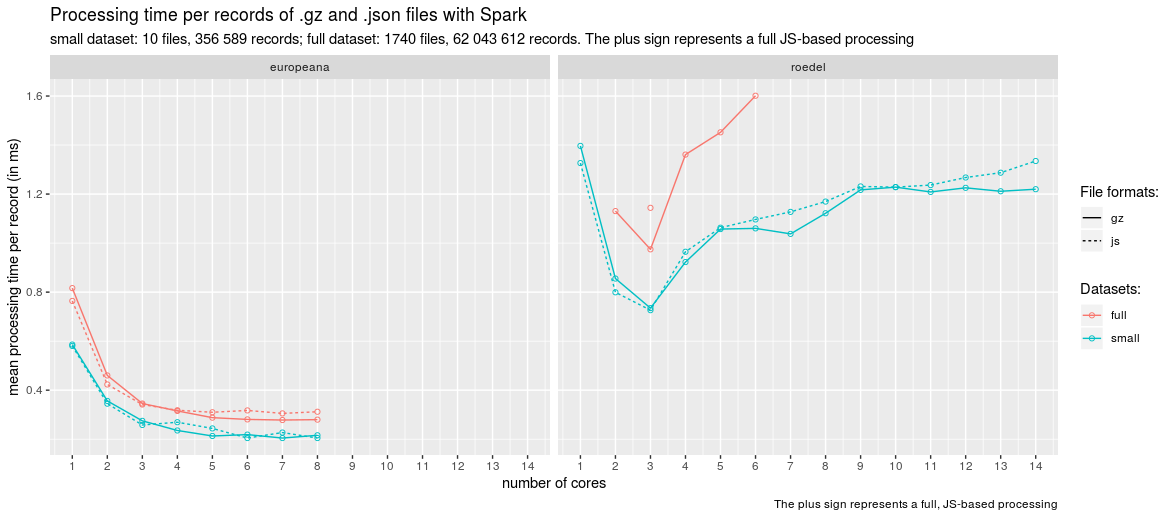
\includegraphics[width=\textwidth]{images/chapter06/small-and-full-measurements-two-servers.png}
\caption{Processing time per records with different settings}
\label{small-and-full-measurements-two-servers}
\end{figure}

1) The per record processing times for the small set is faster. It is not surprising given, that processing time depends on the complexity of the record structure which correlates with the size of the record. It is more important that the shape of the small set and the full set are close to each other, which means that running a small set for this kind of application might predict the running of the full set. An important factor is that the processing function (`measure()') is stateless, the incorporating classes do not collect data (unless in exceptional cases), so the measurement does not depend on previous records. Not all Spark client code works this way, so the statement about the prediction holds only for stateless ones.

2) Gzip compressed files are usually slightly faster than uncompressed. Processing compressed file has two side effects. First, uncompressed files are partitioned, and -- as we saw above -- each partition is paired with a distinct tasks, with its own overhead. Second, decompression also has its own overhead. The evident advantage of using compressed files is sparing of disk space. Note: since on `roedel' machine the full process took more than a day, and we did not had enough machine time, we just run the predictably fastest setting on uncompressed files.

3) The shape of lines on the two machines are significantly different. On `euroepana' the performance is continuously increasing up to 7 cores, but after a given number of cores the improvement is not significant. To find the optimal settings for the number of cores is not easy here, because there is no clear winner. One can decide on two factors, the first one being that the examined speed might be already 'good enough', the second being that while using more cores slightly improves the performance of the current process, it takes resources away from other processes running on the same system, which is an impolite behaviour. On `roedel' the situation is radically different; it has a clear peak at 3 cores. The general reason is that the system throughput (the combination of CPU, memory and I/O operation speed and other factors) has a maximum. If we run more processes parallel some of them consume all the available resources while some others have to wait for moments. To detect the actual bottleneck is not easy, we will see some techniques for this task later.

\subsection{Memory allocation}

The next setting under test is the amount of allocated memory. The process were run on the small, compressed set with different cores and allocating 1, 2, 3, and 4 GB memory for both Spark driver (the central controller) and executors (the parts which execute client code). The spark settings are available in Listing \ref{code:spark-memory}.

\begin{lstlisting}[
  % one can adjust spacing here if required
  % aboveskip=2.5\baselineskip,
  % belowskip=-.8\baselineskip,
  caption={Spark's memory allocation options},
  label=code:spark-memory,
  language=Bash,
  float]
spark-submit --driver-memory <memory> --executor-memory <memory> ...
\end{lstlisting}

\begin{figure}
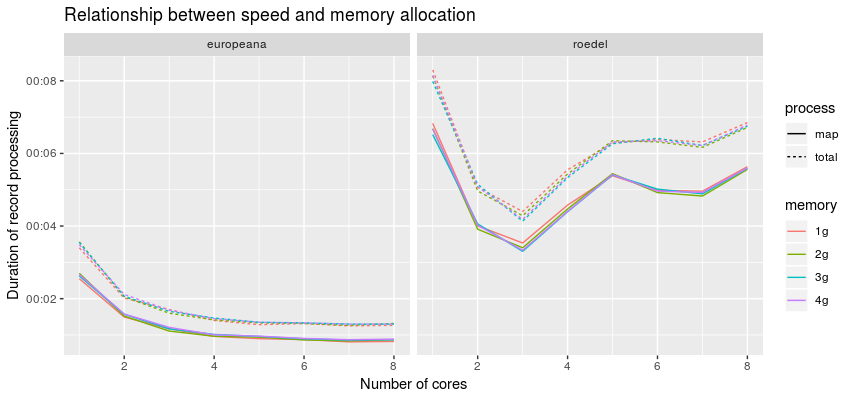
\includegraphics[width=\textwidth]{images/chapter06/memory-allocation-details.png}
\caption{Relationship between speed and memory allocation.}
\label{memory-allocation-details}
\end{figure}

Fig. \ref{memory-allocation-details} shows the result of different memory allocations. Succinctly, these settings do not have any clear effect. It is not a surprise, since the application is virtually stateless. If it would accumulate large (or lots of) variables in memory -- which happens in several Spark SQL or Spark ML based application -- we would see a different graph. The conclusion is that for this application it is not worth to allocate more memory than default (which is 1 GB for the current Spark version).

\subsection{HDFS or normal FS?}

Spark works well with Hadoop Distributed File System (HDFS)\footnote{\url{http://hadoop.apache.org/docs/current/hadoop-project-dist/hadoop-hdfs/HdfsDesign.html}}, but does it perform better in a standalone setup, where HDFS runs on a single machine, and is not distributed over nodes? The Spark settings is available in Listing \ref{code:hdfs}. The result is shown in Fig. \ref{hdfs-vs-fs}.

\begin{lstlisting}[
  % one can adjust spacing here if required
  % aboveskip=2.5\baselineskip,
  % belowskip=-.8\baselineskip,
  caption={Reading from HDFS},
  label=code:hdfs,
  language=Bash,
  float]
spark-submit --inputFileName hdfs://localhost:9000/europeana/*.gz ...
\end{lstlisting}


\begin{figure}
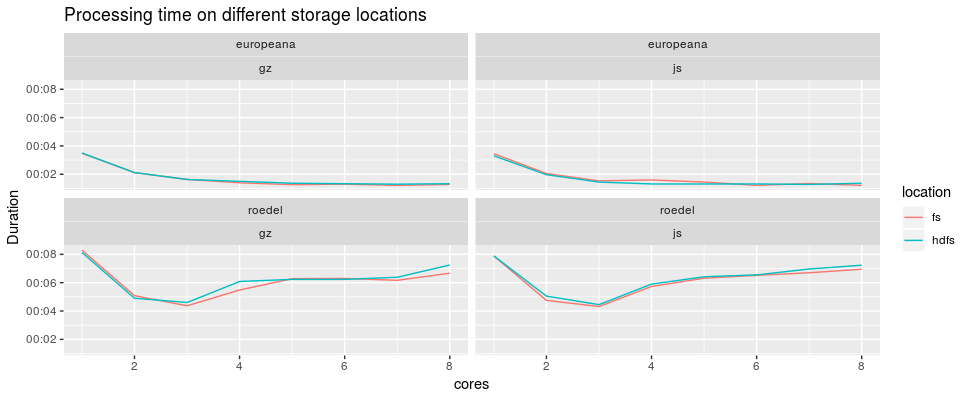
\includegraphics[width=\textwidth]{images/chapter06/hdfs-vs-fs.png}
\caption{Processing time on different storage locations}
\label{hdfs-vs-fs}
\end{figure}

In most cases the results are slightly better for OS file system, but not always, and usually the difference is small. The question whether it is worth to use HDFS or not depends on the speed gain and the cost of the setup of HDFS. In these systems the advantage does not hold, so it is not worth to store files in HDFS.

\section{Event log and history server -- to measure performance}

It was mentioned earlier that Spark launches a monitoring web service (unless it is disabled), which provides useful information about the running process. Although he application is shut down when the process ends, fortunately Spark provides a tool to keep history information persisted. It requires to set a directory into which the application stores the events alongside with their metrics. The history server is similar to the monitoring server, however it process data from the saved event log, and not from the live process. Since the event log is a simple text file containing JSON formatted lines, it is possible to move it and display the content on a different machine.\footnote{The event log file name consists of the master name and the timestamp of the start (such as `local-1550822115584'). This name is also used as an identifier inside the file. If you would like to use it in another machine, rename the file and change its identifier in its content (e.g. in this experiment we used names such as `europeana-c4').} It is very important to note that the web interface does not show all the information from the event log. History server provides an API, so the data could be programmatically read from it.

\begin{lstlisting}[
  % one can adjust spacing here if required
  % aboveskip=2.5\baselineskip,
  % belowskip=-.8\baselineskip,
  caption={Spark history server setting and launch},
  label=code:history-server,
  language=Bash,
  float]
> cd $SPARK_HOME
> more conf/spark-defaults.conf
...
spark.eventLog.enabled         true
spark.eventLog.dir             file:/path/to/spark-event-log
spark.history.fs.logDirectory  file:/path/to/spark-event-log
> sbin/start-history-server.sh
\end{lstlisting}

\begin{figure}
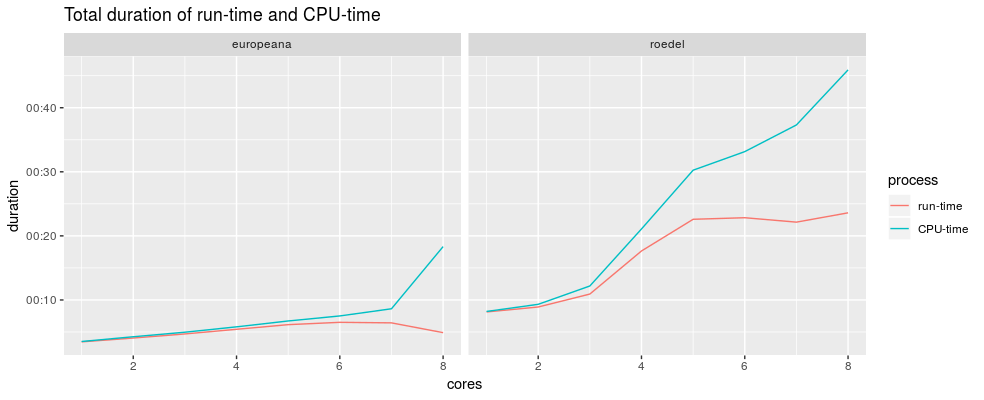
\includegraphics[width=\textwidth]{images/chapter06/runtime-vs-cputime-absolute.png}
\caption{Processing time on different storage locations}
\label{runtime-vs-cputime-absolute}
\end{figure}

The most important information for our experiment are `executorRunTime' and `executorCpuTime' variables. According to Spark API documentation \cite{spark-taskmetrics} `executorRunTime' is the "time the executor spends actually running the task (including fetching shuffle data)", while `executorCpuTime' is the "CPU Time the executor spends actually running the task (including fetching shuffle data) in nanoseconds". Since our process does not have shuffle steps, we can suppose that most of the time happens inside the map() function. According to \cite{canali2017} the difference between run-time and CPU-time is the time the CPU waits for the memory. Fig. \ref{runtime-vs-cputime-absolute} reveals that this time is getting larger and larger in both machines as we increase the number of cores. It is natural, because more and more process should compete for the resources. The two machines behave differently regarding to the increasing of this difference between times.

\begin{figure}
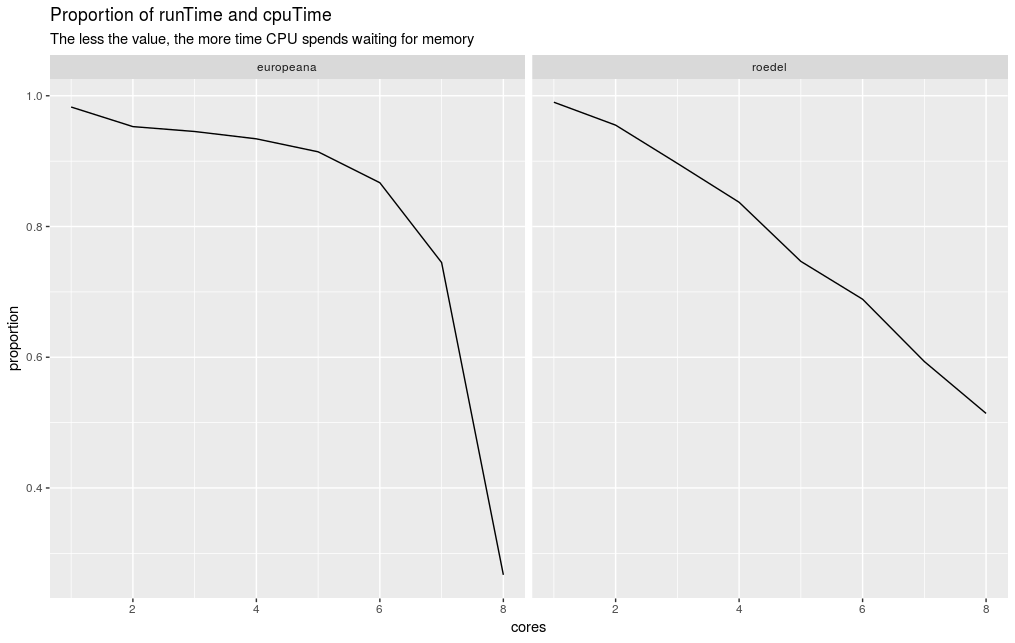
\includegraphics[width=\textwidth]{images/chapter06/runtime-vs-cputime.png}
\caption{Proportion of run-time and CPU-time. The larger the distance, the more time CPU is waiting.}
\label{runtime-vs-cputime}
\end{figure}

If we display it differently, highlighting the relative numbers i.e. the proportion of run-time and CPU-time in Fig. \ref{runtime-vs-cputime}, we see an interesting pattern. While in `europeana' the degradation is moderated up until 6 cores and from then progressive, on `roedel' it is linear. It means that the CPU is waiting a lot even when it performs well under small number of cores.

\begin{figure}
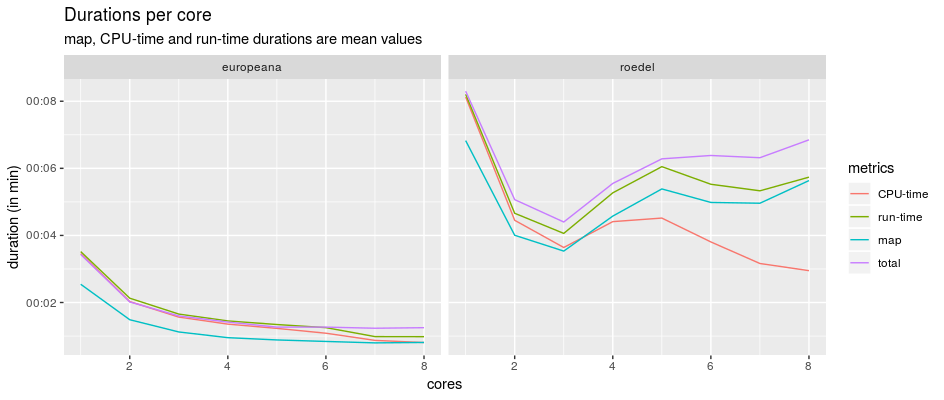
\includegraphics[width=\textwidth]{images/chapter06/all-durations.png}
\caption{Duration of different components per CPU.}
\label{all-durations}
\end{figure}

In the last figure (Fig. \ref{all-durations}) along with run-time and CPU-time the time of map method and the total time is also displayed. It reveals the reason of the performance peak: the best performance happens before the time of map exceeds the CPU-time. It is not clear exactly what other processes involved in the task, but it is clear, that CPU does other things as well, because up to that crossing CPU-time is larger then map-time. But when map-time gets bigger than CPU-time, it is clear that map (and the other confounded processes) has to wait for free memory. This crossing happened on `europeana' between 7 and 8 cores, while on `roedel' between 3 and 4 cores. It is also interesting that at 8 cores on `roedel' the map-time is almost reach run-time, and almost half of it is spent for waiting.

One last note about the hidden processes. As mentioned earlier Spark optimizes its code, and it is not the high level API which finally runs in the JVM. Another important feature of this API is that the methods are classified either as transformations or as actions. In Spark nothing happens until an action triggers the launch of the processing workflow, in which the transformations happen in a pipeline manner. It has two important consequences. First, the duration of some methods can not be measured in the client code, because it only assembles the building blocks, but not runs it. Second, there is no clear mapping between client code, and what a Java profiler shows, not just because of the optimization process, but also because of intensive usage of language constructions such as lambda functions. For example textFile() method which reads the file is not shown up in the Java stack trace.

\section{Conclusion}

The most important lessons learned in this experiment is that allocating more resources does not necessary imply better performance, and what we really need in an environment with limited and shared resources is a `good enough' state which politely let other processes run. To find the optimal settings it is suggested to pick up a smaller sample, which is similar to the full dataset in important characteristics, and measure speed with different settings. The settings worth to check are number of cores, memory allocation, compression of the source files, and different file systems (if they are available). As a source of ground truth one can use Spark log (which contains some performance indicator), Spark event log (disabled by default), or measuring points in your application (via Spark accumulators \cite{spark-accumulators}).

% \bibliographystyle{acm}
% \bibliography{bibliography-for-papers}
